\documentclass[12pt]{beamer}
\usepackage[utf8]{inputenc}
%\usepackage[latin1]{inputenc}
\usepackage[spanish]{babel}
%\usetheme{Warsaw}
%\usepackage{euler}
\usepackage{amsmath}
\usepackage{amsthm}
\usepackage{multicol}
\usepackage{graphicx}
\usepackage{tikz}
\usepackage{color}
\usepackage{listings}
\lstset{ %
language=C++,                % choose the language of the code
basicstyle=\footnotesize,       % the size of the fonts that are used for the code
numbers=left,                   % where to put the line-numbers
numberstyle=\footnotesize,      % the size of the fonts that are used for the line-numbers
stepnumber=1,                   % the step between two line-numbers. If it is 1 each line will be numbered
numbersep=5pt,                  % how far the line-numbers are from the code
backgroundcolor=\color{white},  % choose the background color. You must add \usepackage{color}
showspaces=false,               % show spaces adding particular underscores
showstringspaces=false,         % underline spaces within strings
showtabs=false,                 % show tabs within strings adding particular underscores
frame=single,   		% adds a frame around the code
tabsize=2,  		% sets default tabsize to 2 spaces
captionpos=b,   		% sets the caption-position to bottom
breaklines=true,    	% sets automatic line breaking
breakatwhitespace=false,    % sets if automatic breaks should only happen at whitespace
escapeinside={\%}{)}          % if you want to add a comment within your code
}
%\usepackage{epstopdf}
\DeclareGraphicsExtensions{.pdf,.png,.jpg}
\renewcommand {\arraystretch}{1.5}
\mode<presentation>
{
  \usetheme{CambridgeUS}
  \setbeamercovered{transparent}
  % or whatever (possibly just delete it)
}
\title{Tema 0 - Programaci\'{o}n b\'{a}sica con Python}
\subtitle{Curso de F\'{i}sica Computacional}
\author{M. en C. Gustavo Contreras May\'{e}n}
\date{9 de agosto de 2012}
%\email{curso.fisica.comp@gmail.com}
%\ptsize{10}
\begin{document}
\maketitle
\fontsize{14}{14}\selectfont
\spanishdecimal{.}
\begin{frame}{Contenido}
\tableofcontents[pausesections]
\end{frame}
\section{Introducci\'{o}n}
\begin{frame}
Para el curso de F\'{i}sica Computacional ser\'{a} necesario que usemos un lenguaje de programaci\'{o}n para apoyarnos en la soluci\'{o}n de los problemas y algoritmos.
\\
\bigskip
El lenguaje de nuestra elecci\'{o}n es un medio para alcanzar nuestro objetivo del curso, m\'{a}s no el fin, por lo que revisaremos lo m\'{a}s b\'{a}asico de Python, dando la oportunidad de que por tu cuenta, logres un mayor conocimiento y pr\'{a}ctica con Python.
\end{frame}
\begin{frame}
\begin{figure}
	\centering
	
\includegraphics[scale=0.5]{python-logo-master-v3-TM2.eps} 
\end{figure}
\begin{itemize}
\item Lenguaje de programaci\'{o}n de alto nivel, interpretado.
\item Desarrollado por Guido van Rossum a principios de
los años 90.
\item Es multiplataforma (UNIX, Solaris, Linux, DOS, Windows, OS/2, Mac OS, etc.)
\item Software libre: Python Software Foundation License (PSFL)
\item Tipado din\'{a}mico.
\item Fuertemente tipado.
\item Orientado a objetos.
\end{itemize}
\end{frame}
\begin{frame}
\frametitle{Tipado din\'{a}mico}
Cada dato es de un tipo determinado y s\'{o}lo se puede operar con \'{e}l de formas bien definidas.
\\
\bigskip
La ventaja es que \textcolor{red}{NO hay que declarar variables antes de
su uso}.
\end{frame}
\begin{frame}
\frametitle{Fuertemente tipado}
Se dice que es un lenguaje cuyos tipos son estrictos. Java y Python son fuertemente tipados.
\\
\bigskip
Si tiene un tipo de dato entero, no puede tratarlo como una cadena de texto sin convertirlo expl\'{i}citamente.
\end{frame}
\begin{frame}
\frametitle{Programaci\'{o}n orientada a objetos}
La programaci\'{o}n orientada a objetos es un paradigma de programaci\'{o}n que busca representar entidades u objetos agrupando datos y m\'{e}todos que puedan describir sus caracter\'{i}sticas y comportamientos.
\end{frame}
\begin{frame}
\frametitle{Complementos para Python}
\begin{itemize}
\item NumPy: paquete fundamental para computaci\'{o}n cient\'{i}fica.
\item SciPy: librer\'{i}a para computaci\'{o}n cient\'{i}fica (extiende a NumPy)
\item matplotlib: librer\'{i}a para gr\'{a}ficos 2D (soporta gr\'{a}ficos 3D tambi\'{e}n)
\item Mayavi: librer\'{i}a para gr\'{a}ficos y visualizaci\'{o}n de datos 3D.
\item iPython: consola interactiva para Python.
\end{itemize}
\end{frame}
\begin{frame}
\begin{figure}
	\centering
	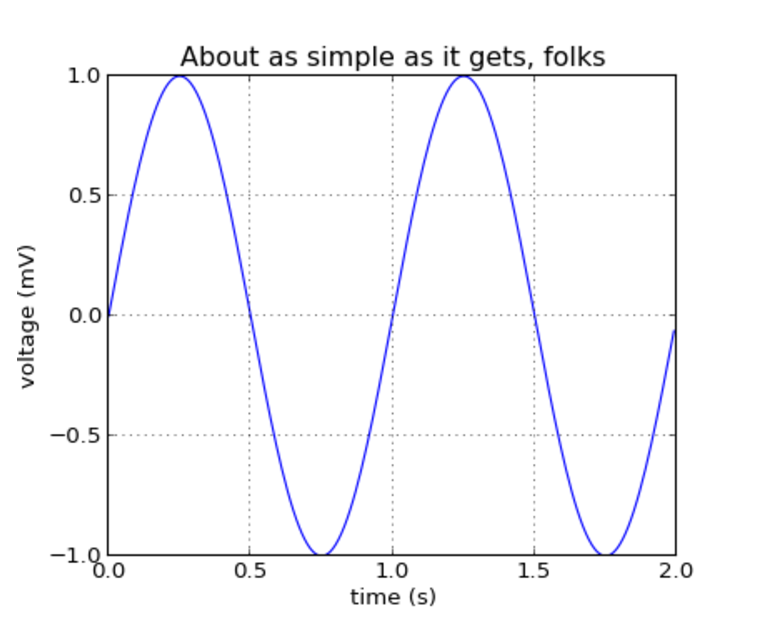
\includegraphics[scale=0.5]{simple_plot1.eps}<1> 
	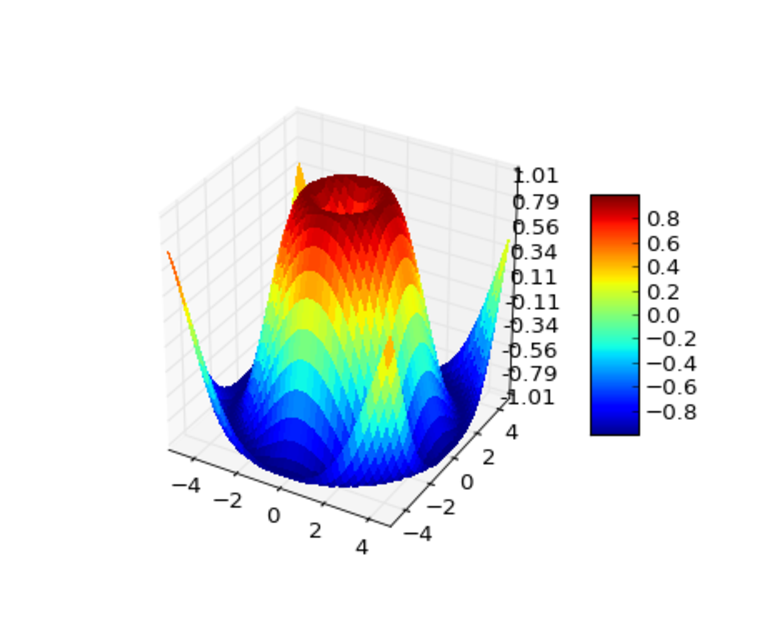
\includegraphics[scale=0.5]{surface3d_demo4.eps}<2>
	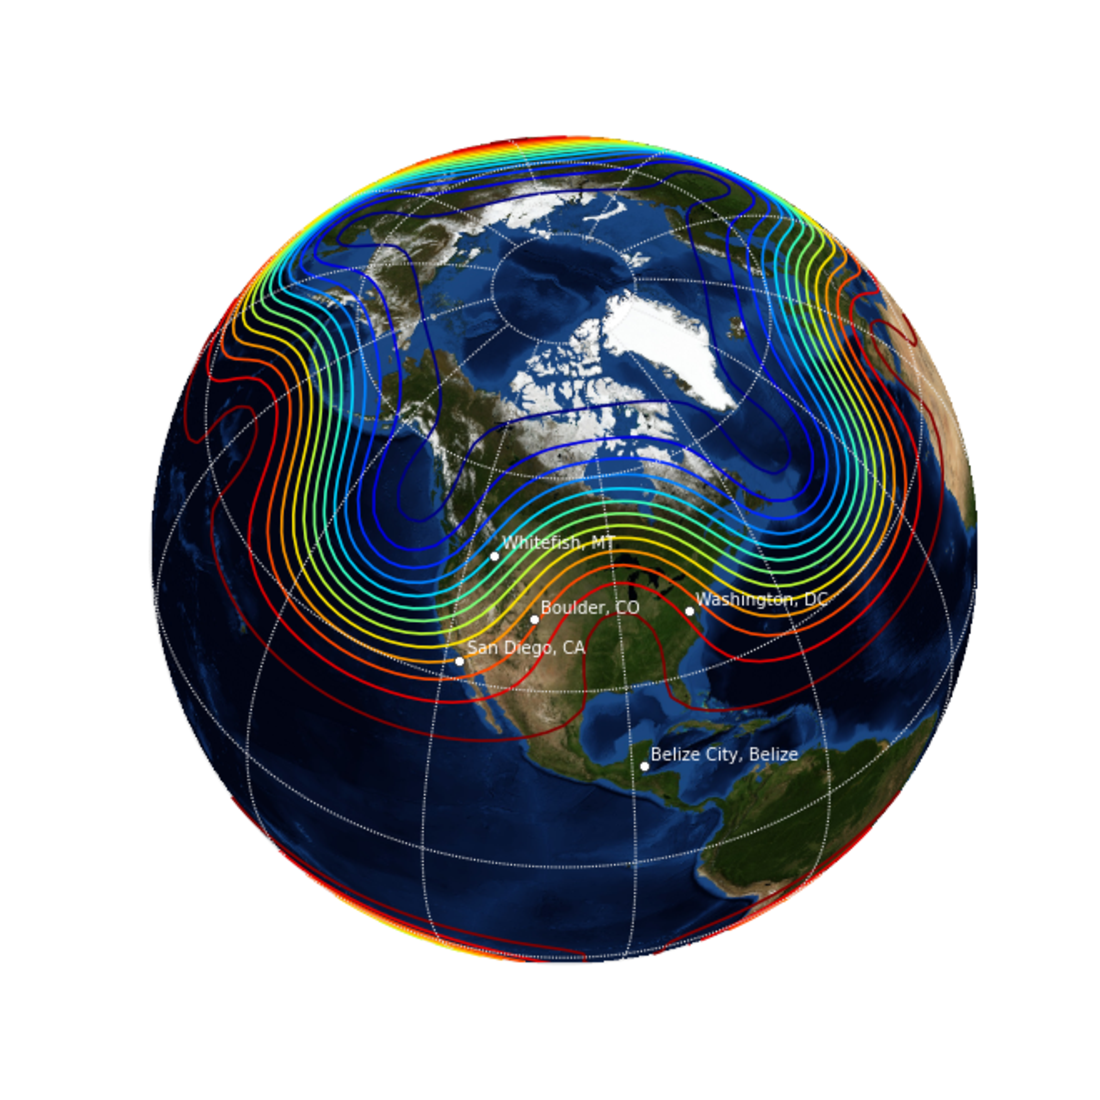
\includegraphics[scale=0.5]{plotmap.eps}<3>
\end{figure}
\end{frame}
\section{Iniciando con Python}
\begin{frame}
\frametitle{Consola de trabajo en Python}
Hay dos modos de trabajo en Python, cada uno de ellos depende de nuestra habilidad:
\begin{itemize}
\item \textbf{Modo rudo}: trabajo directo en la consola.
\item \textbf{Modo amigable}: a trav\'{e}s de una interface IDLE (Entorno de Desarrollo Integrado)
\end{itemize}
\end{frame}
\begin{frame}
\frametitle{Modo Rudo}
\begin{figure}
	\centering
	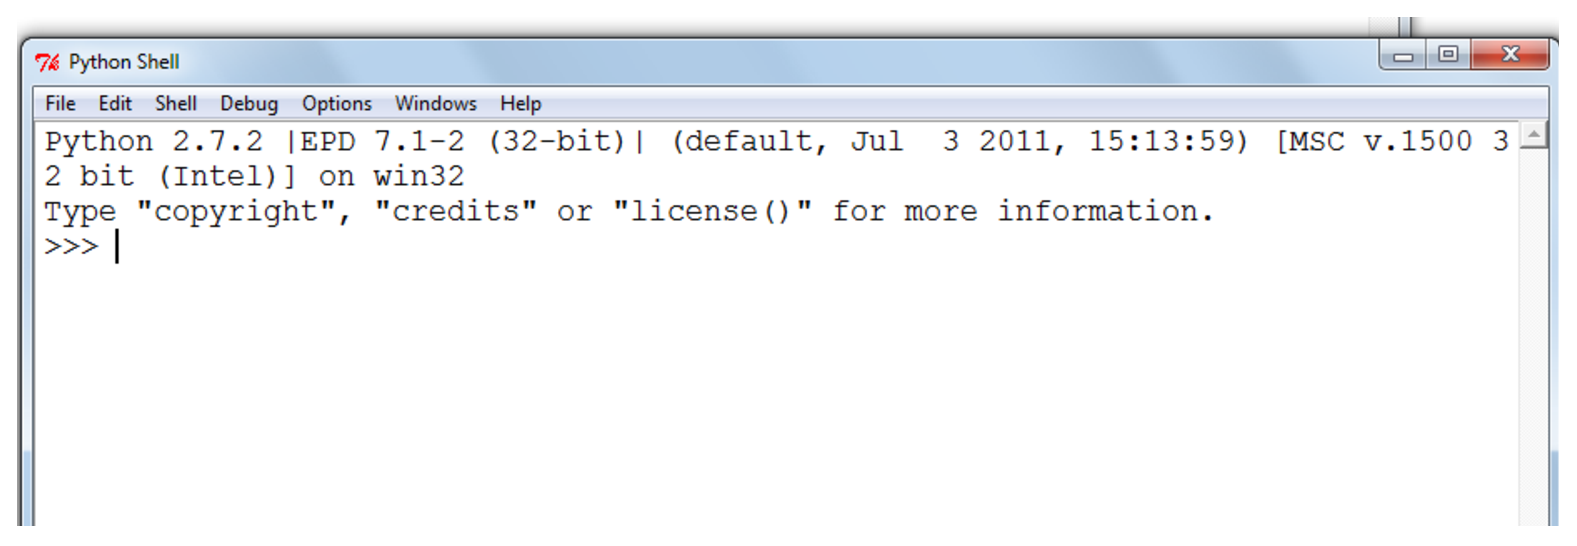
\includegraphics[scale=0.5]{pantalla01.eps} 
\end{figure}
\end{frame}
\begin{frame}
\frametitle{Python como calculadora}
Una vez abierta la sesi\'{o}n en Python, podemos aprovechar al m\'{a}ximo Python, una de las primeras facilidades que tenemos, es que contamos con una calculadora a la mano, s\'{o}lo hay que ir escribiendo las operaciones.
\end{frame}
\begin{frame}[fragile]
\frametitle{Operadores artim\'{e}ticos}
\begin{minipage}{5.5cm}
\begin{exampleblock}{}<1->
	\verb|>>> 3+4| \\
	\pause
	\textcolor{blue}{\texttt{7}}
\end{exampleblock}
\begin{exampleblock}{}<2->
	\verb|>>> 3/4| \\
	\pause
	\textcolor{blue}{\texttt{0}}
\end{exampleblock}
\begin{exampleblock}{}<3->
	\verb|>>> 3.0/4.0| \\
	\pause
	\textcolor{blue}{\texttt{0.75}}
\end{exampleblock}
\begin{exampleblock}{}<4->
	\verb|>>> 5.0 / 10 * 2 + 5| \\
	\pause
	\textcolor{blue}{\texttt{6}}
\end{exampleblock}
\end{minipage}
\hspace{0.5cm}
\begin{minipage}{5.5cm}
\begin{exampleblock}{}<5->
	\verb|>>> 5.0 / (10 * 2 + 5)| \\
	\pause
	\textcolor{blue}{\texttt{0.2}}
\end{exampleblock}
\begin{exampleblock}{}<6->
	\verb|>>> 2**3**2| \\
	\pause
	\textcolor{blue}{\texttt{512}}
\end{exampleblock}
\begin{exampleblock}{}<7->
	\verb|>>> (2**3)**2| \\
	\pause
	\textcolor{blue}{\texttt{64}}
\end{exampleblock}
\begin{exampleblock}{}<8->
	\verb|>>> 17%3%2| \\
	\pause
	\textcolor{blue}{\texttt{0}}
\end{exampleblock}
\end{minipage}
\end{frame}
\begin{frame}
\frametitle{Tabla de operadores}
\begin{center}
\begin{tabular}{| c | c | c | c |}
\hline
Operador & Operaci\'{o}n & Ejemplo & Resultado \\
\hline
\hline
$**$ & Potencia & $2**3$ & $8$ \\
$*$ & Multiplicaci\'{o}n & $7*3$ & 21 \\
$/$ & Divisi\'{o}n & $10.5/2$ & 5.25 \\
$//$ & Divisi\'{o}n entera & $10.5//2$ & 5.0 \\
$+$ & Suma & $3+4$ & $7$ \\
$-$ & Resta & $6-8$ & $-2$ \\
$\%$ & M\'{o}dulo & $15\%6$ & $3$ \\
\hline
\end{tabular}
\end{center}
\end{frame}
\begin{frame}
\frametitle{Precedencia de operadores 1}
\begin{enumerate}
\item Las expresiones contenidas dentro de pares de par\'{e}ntesis son evaluadas primero. En el caso de expresiones con par\'{e}ntesis anidados, los operadores en el par de par\'{e}ntesis m\'{a}s interno son aplicados primero.
\item Las operaciones de exponentes son aplicadas despu\'{e}s. Si una expresi\'{o}n contiene muchas operaciones de exponentes, los operadores son aplicados de derecha a izquierda.
\end{enumerate}
\end{frame}
\begin{frame}
\frametitle{Precedencia de operadores 2}
\begin{enumerate}
\setcounter{enumi}{2}
\item La multiplicaci\'{o}n, divisi\'{o}n y m\'{o}dulo son las siguientes en ser aplicadas. Si una expresi\'{o}n contiene muchas multiplicaciones, divisiones u operaciones de m\'{o}dulo, los operadores se aplican de izquierda a derecha.
\item Suma y resta son las operaciones que se aplican por \'{u}ltimo. Si una expresi\'{o}n contiene muchas operaciones de suma y resta, los operadores son aplicados de izquierda a derecha. La suma y resta tienen el mismo nivel de precedencia.
\end{enumerate}
\end{frame}
\section{Operadores relacionales}
\begin{frame}[fragile]
\frametitle{Operadores relacionales (de comparaci\'{o}n}
Tipos de datos l\'{o}gicos: \texttt{False (0)} y \texttt{True (1)}
\begin{minipage}{5.5cm}
\begin{exampleblock}{}<1->
	\verb|1+2>7-3| \\
	\pause
	\textcolor{blue}{\texttt{False}}
\end{exampleblock}
\begin{exampleblock}{}<2->
	\verb|1<2<3| \\
	\pause
	\textcolor{blue}{\texttt{True}}
\end{exampleblock}
\begin{exampleblock}{}<3->
	\verb|1>2==2<3| \\
	\pause
	\textcolor{blue}{\texttt{False}}
\end{exampleblock}
\begin{exampleblock}{}<4->
	\verb|1>(2==2)<3| \\
	\pause
	\textcolor{blue}{\texttt{False}}
\end{exampleblock}
\end{minipage}
\hspace{0.5cm}
\begin{minipage}{5.5cm}
\begin{exampleblock}{}<5->
	\verb|3>4<5| \\
	\pause
	\textcolor{blue}{\texttt{False}}
\end{exampleblock}
\begin{exampleblock}{}<6->
	\verb|1.0/3<0.33333| \\
	\pause
	\textcolor{blue}{\texttt{False}}
\end{exampleblock}
\begin{exampleblock}{}<7->
	\verb|5.0/3>=11/7.0| \\
	\pause
	\textcolor{blue}{\texttt{True}}
\end{exampleblock}
\begin{exampleblock}{}<8->
	\verb|2**(2/3)<3**(3/4)| \\
	\pause
	\textcolor{blue}{\texttt{False}}
\end{exampleblock}
\end{minipage}
\end{frame}
\begin{frame}
\frametitle{Tabla de operadores relacionales}
\begin{center}
\begin{tabular}{| c | c | c | c |}
\hline
Operador & Operaci\'{o}n & Ejemplo & Resultado \\
\hline
\hline
$==$ & Igual a & $4==5$ & \texttt{False}  \\
$!=$ & Diferente de & $2!=3$ & \texttt{True} \\
$<$ & Menor que & $10<4$ & \texttt{False} \\
$>$ & Mayor que & $5>-4$ & \texttt{True} \\
$>=$ & Menor o igual que & $7<=7$ & \texttt{True} \\
$>=$ & Mayor o igual que & $3.5 >= 10$ & \texttt{False} \\
\hline
\end{tabular}
\end{center}
\end{frame}
\begin{frame}
\frametitle{Operadores l\'{o}gicos (booleanos)}
\begin{center}
\begin{tabular}{| c | c | c | c |}
\hline
Operador & Operaci\'{o}n & Ejemplo & Resultado \\
\hline
\hline
\texttt{and} & conjunci\'{o}n & \texttt{False and True} & \texttt{False} \\
\texttt{or} & disyunci\'{o}n & \texttt{False or True} & \texttt{True} \\
\texttt{not} & negaci\'{o}n & \texttt{not True} & \texttt{False} \\
\hline
\end{tabular}
\end{center}
\end{frame}
\begin{frame}
\frametitle{Tabla de verdad}
\texttt{
\begin{center}
\begin{tabular}{| c | c | c | c | c |}
\hline
A & B & A and B & A or B & not A \\
\hline
\hline
True & True & True & True & True \\
True & False & False & True & False \\
False & True & False & True & True \\
False & False & False & False & True \\
\hline
\end{tabular}
\end{center}
}
\end{frame}
\begin{frame}
\frametitle{Tipos de datos}
Cada lenguaje de programaci\'{o}n requiere de un conjunto de tipos de datos para operar, cada uno est\'{a} caracterizado por un nombre, un tamaño de espacio en memoria y un intervalo.
\\
\bigskip
Realizar operaciones entre diferentes tipos de datos nos va a generar un error, ya que como hemos mencionado, Python es un lenguaje fuertemente tipado, moraleja: sumar peras con peras y manzanas con manzanas.
\end{frame}
\begin{frame}
\frametitle{Tabla de tipos de datos}
\fontsize{8}{8}\selectfont
\begin{center}
\begin{tabular}{c c c c c}
\hline
Tipo & Descripci\'{o}n & bits & Rango & Ejemplo \\
\hline
\texttt{bol} & booleano & $8$ & sin rango & \texttt{True} o \texttt{False} \\
\texttt{int} & entero & $16$ & $[-2^{15}, 2^{15}-1]$ & $327$ \\
\texttt{long int} & entero largo & $32$ & $[0, 2^{32}-1]$ & $24334253234L$ \\
 \texttt{float} & real (punto flotante) & $32$ & $[-2^{31}, 2^{31}-1]$ & $3.1416$ \\
 \texttt{string} & string (cadena) & $32$ & $[-2^{31}, 2^{31}-1]$ & 'hola' \\
\texttt{tuple} & tupla & $32$ & $[3.4 \times 10^{-38}, 3.4 \times 10^{38}]$ & \texttt{1, 'aja',2.0)} \\
\texttt{list} & lista & $64$ & $[1.7 \times 10^{-308}, 1.7 \times 10^{308}]$ & \texttt{[1, 'aja', 2.0]} \\
\texttt{dict} & diccionario & 80 & $[3.4 \times 10^{-4932}, 3.4 \times 10^{4932}]$ & \texttt{'a':7.0, 23: True}
\end{tabular}
\end{center}
\end{frame}
\begin{frame}
\frametitle{Palabras reservadas}
No se pueden utilizar dentro del c\'{o}digo
\fontsize{12}{12}\selectfont
\begin{multicols}{6}
\texttt{and \\
del \\
for \\
is \\
raise \\
assert \\
elif \\
from \\
lambda \\
return \\
break \\
else \\
global \\
not \\
try \\
class \\
except \\
if \\
or \\ 
while \\
continue \\
exec \\
import \\
pass \\
yield \\
def \\
finally \\
in \\
print \\
del 
}
\end{multicols}
\end{frame}
\begin{frame}
\frametitle{Identificadores}
Son nombres que hacen referencia a los objetos que componen un programa: constantes, variables, funciones, etc.
\\
\bigskip
Reglas para construir identificadores:
\begin{enumerate}
\item El primer car\'{a}cter debe ser una letra o el car\'{a}cter de subrayado (gui\'{o}n bajo)
\item El primer car\'{a}cter puede ir seguido de un n\'{u}mero variable de d\'{i}gitos num\'{e}ricos, letras o car\'{a}cteres de subrayado.
\item No pueden utilizarse espacios en blanco, ni s\'{i}mbolos de puntuaci\'{o}n.
\item Python distingue may\'{u}sculas y min\'{u}sculas.
\item No pueden utilizarse palabras reservadas del lenguaje.
\end{enumerate}
\end{frame}
\section{Variables}
\begin{frame}[fragile]
\frametitle{Variables}
\fontsize{10}{10}\selectfont
\begin{minipage}{5.5cm}
\begin{exampleblock}{}<1->
 \verb|>>> base = 2| \\
\end{exampleblock}
\begin{exampleblock}{}<2->
 \verb|>>> print base| \\
 \pause
 \textcolor{blue}{2}
\end{exampleblock}
\begin{exampleblock}{}<3->
 \verb|>>> print "base"| \\
 \pause 
 \textcolor{blue}{\texttt{base}}
\end{exampleblock}
\begin{exampleblock}{}<4->
 \verb|>>> base = base + 1|
\end{exampleblock}
\end{minipage}
\hspace{0.5cm}
\begin{minipage}{5.5cm}
\begin{exampleblock}{}<5->
 \verb|>>> base| \\
 \pause
 \textcolor{blue}{3}
\end{exampleblock}
\begin{exampleblock}{}<6->
 \verb|>>> alt = 4| \\
\end{exampleblock}
\begin{exampleblock}{}<7->
 \verb|>>> area = base+alt; a= 3|
\end{exampleblock}
\begin{exampleblock}{}<8->
 \verb|>>> a= 2*a| \\
\end{exampleblock}
\end{minipage}
\end{frame}
\begin{frame}[fragile]
\fontsize{12}{12}\selectfont
\begin{minipage}{5.5cm}
\begin{exampleblock}{}<1->
 \verb|>>> area== 2*a| \\
 \pause
 \textcolor{blue}{\texttt{False}}
\end{exampleblock}
\begin{exampleblock}{}<2->
 \verb|>>> x= "uno"; y= "dos"| \\
\end{exampleblock}
\begin{exampleblock}{}<3->
 \verb|>>> x| \\
 \pause
 \textcolor{blue}{\texttt{uno}}
\end{exampleblock}
\begin{exampleblock}{}<4->
 \verb|>>> print x| \\
 \pause
 \textcolor{blue}{\texttt{uno}}
\end{exampleblock}
\end{minipage}
\hspace{0.5cm}
\begin{minipage}{5.5cm}
\begin{exampleblock}{}<5->
 \verb|>>> x+y| \\
 \pause
 \textcolor{blue}{\texttt{unodos}}
\end{exampleblock}
\begin{exampleblock}{}<6->
 \verb|>>> print x+y| \\
 \pause
 \textcolor{blue}{\texttt{unodos}}
\end{exampleblock}
\end{minipage}
\end{frame}
\section{Listas y Tuplas}
\begin{frame}[fragile]
\frametitle{Listas y Tuplas}
\fontsize{12}{12}\selectfont
\begin{minipage}{5.5cm}
\begin{exampleblock}{}<1->
	\verb|milista=[a,"hola",3.0,True]|
\end{exampleblock}
\begin{exampleblock}{}<2->
	\verb|milista| \\
	\pause
	\textcolor{blue}{\texttt{[8,"hola",3.0,True]}}
\end{exampleblock}
\begin{exampleblock}{}<3->
	\verb|milista[0]| \\
	\pause
	\textcolor{blue}{\texttt{8}}
\end{exampleblock}
\begin{exampleblock}{}<4->
	\verb|milista[1]| \\
	\pause
	\textcolor{blue}{\texttt{'hola'}}
\end{exampleblock}
\begin{exampleblock}{}<5->
	\verb|milista[2]| \\
	\pause
	\textcolor{blue}{\texttt{3.0}}
\end{exampleblock}
\end{minipage}
\hspace{0.5cm}
\begin{minipage}{5.5cm}
\begin{exampleblock}{}<6->
	\verb|milista[1:3]| \\
	\pause
	\textcolor{blue}{\texttt{'hola',3.0}}
\end{exampleblock}
\begin{exampleblock}{}<7->
	\verb|milista[0] = 2.0|
\end{exampleblock}
\begin{exampleblock}{}<8->
	\verb|milista| \\
	\pause
	\textcolor{blue}{\texttt{[2.0,"hola",3.0,True]}}
\end{exampleblock}
\begin{exampleblock}{}<9->
	\verb|milista[-1]| \\
	\pause
	\textcolor{blue}{\texttt{True}}
\end{exampleblock}
\end{minipage}
\end{frame}
\begin{frame}[fragile]
\fontsize{10}{10}\selectfont
\begin{minipage}{5.5cm}
\begin{exampleblock}{}<1->
	\verb|milista.append("otro")| \\
\end{exampleblock}
\begin{exampleblock}{}<2->
	\verb|milista| \\
	\pause
	\textcolor{blue}{\texttt{[2.0,"hola",3.0,True,'otro']}}
\end{exampleblock}
\begin{exampleblock}{}<3->
	\verb|milista[:2]| \\
	\pause
	\textcolor{blue}{\texttt{[2.0,"hola"]}}
\end{exampleblock}
\begin{exampleblock}{}<4->
	\verb|milista[1:]| \\
	\pause
	\textcolor{blue}{\texttt{[2.0,"hola",3.0,True]}}
\end{exampleblock}
\begin{exampleblock}{}<5->
	\verb|lista2=[]|
\end{exampleblock}
\end{minipage}
\hspace{0.5cm}
\begin{minipage}{5.5cm}
\begin{exampleblock}{}<6->
	\verb|lista2| \\
	\pause
	\verb|[]|
\end{exampleblock}
\begin{exampleblock}{}<7->
	\verb|lista2.insert(1,"a")|
\end{exampleblock}
\begin{exampleblock}{}<8->
	\verb|lista2| \\
	\pause
	\textcolor{blue}{\texttt{['a']}}
\end{exampleblock}
\begin{exampleblock}{}<9->
	\verb|lista2.insert(2,"b")|
\end{exampleblock}
\end{minipage}
\end{frame}
\begin{frame}[fragile]
\begin{minipage}{5.5cm}
\begin{exampleblock}{}<1->
	\verb|lista2| \\
	\pause
	\textcolor{blue}{\texttt{['a','b']}}
\end{exampleblock}
\begin{exampleblock}{}<2->
	\verb|lt = ( 1,2,True, "python" )|
\end{exampleblock}
\end{minipage}
\hspace{0.5cm}
\begin{minipage}{5.5cm}
\begin{exampleblock}{}<3->
	\verb|lt| \\
	\pause
	\textcolor{blue}{\texttt{(1,2, True, 'python' )}}
\end{exampleblock}
\begin{exampleblock}{}<4->
	\verb|lt[0]=3| \\
	\pause
	\textcolor{blue}{\texttt{Ups, hay un error!}}
\end{exampleblock}
\begin{exampleblock}{}<5->
	\verb|3 in lt| \\
	\pause
	\textcolor{blue}{\texttt{False}}
\end{exampleblock}
\end{minipage}
\end{frame}
\begin{frame}[fragile]
\frametitle{Funci\'{o}n \texttt{range}}
La funci\'{o}n \texttt{range()} crea una lista de n\'{u}meros enteros en sucesi\'{o}n aritm\'{e}tica. La funci\'{o}n \texttt{range()} puede tener uno, dos o tres argumentos num\'{e}ricos.
\\
\bigskip
La funci\'{o}n con un \'{u}nico argumento se escribe \texttt{range(n)} y crea una lista creciente de $n$ t\'{e}rminos enteros que empieza en $0$ y acaba en $n-1$ (el incremento es unitario)
\fontsize{12}{12}\selectfont
\begin{minipage}{6cm}
\begin{exampleblock}{}<1->
	\verb|range(8)| \\
	\pause
	\textcolor{blue}{[0,1,2,3,4,5,6,7]}
\end{exampleblock}
\begin{exampleblock}{}<2->
	\verb|range(3,7)| \\
	\pause
	\textcolor{blue}{[3,4,5,6]}
\end{exampleblock}
\end{minipage}
\hspace{0.2cm}
\begin{minipage}{6cm}
\begin{exampleblock}{}<3->
	\verb|range(4,10,2)| \\
	\pause
	\textcolor{blue}{[4,6,8]}
\end{exampleblock}
\end{minipage}
\end{frame}
\begin{frame}[fragile]
\frametitle{Funciones intr\'{i}nsecas}
\fontsize{12}{12}\selectfont
\begin{minipage}{5.5cm}
\begin{exampleblock}{}<1->
	\verb|x =  -5|
\end{exampleblock}
\begin{exampleblock}{}<2->
	\verb|y =  4|
\end{exampleblock}
\begin{exampleblock}{}<3->
	\verb|p =  3.1416|
\end{exampleblock}
\begin{exampleblock}{}<4->
	\verb|z =  '6.3'|
\end{exampleblock}
\begin{exampleblock}{}<5->
	\verb|print int(p)| \\
	\pause
	\textcolor{blue}{3}
\end{exampleblock}
\begin{exampleblock}{}<6->
	\verb|abs(x)| \\
	\pause
	\textcolor{blue}{5}
\end{exampleblock}
\end{minipage}
\hspace{0.5cm}
\begin{minipage}{5.5cm}
\begin{exampleblock}{}<7->
	\verb|print float(z)| \\
	\pause
	\textcolor{blue}{6.0}
\end{exampleblock}
\begin{exampleblock}{}<8->
	\verb|complex(x)| \\
	\pause
	\textcolor{blue}{\texttt{(-5+0j)}}
\end{exampleblock}
\begin{exampleblock}{}<9->
	\verb|complex(x,y)| \\
	\pause
	\textcolor{blue}{\texttt{(-5+4j)}}
\end{exampleblock}
\begin{exampleblock}{}<10->
	\verb|print round(p,2)| \\
	\pause
	\textcolor{blue}{3.14}
\end{exampleblock}
\begin{exampleblock}{}<11->
	\verb|cmp(x,y)| \\
	\pause
	\textcolor{blue}{-1}
\end{exampleblock}
\end{minipage}
\end{frame}
\begin{frame}
\fontsize{12}{12}\selectfont
\begin{center}
\begin{tabular}{| c | c |}
\hline
Operaci\'{o}n & Descripci\'{o}n \\
\hline \texttt{int(x)} & Convierte \texttt{x} a entero \\
\hline \texttt{long(x)} & Convierte \texttt{x} a entero largo \\
\hline \texttt{float(x)} & Convierte \texttt{x} a punto flotante \\
\hline \texttt{complex(x)} & Convierte \texttt{x} al complejo \texttt{x+0j} \\
\hline \texttt{complex(x,y)} & Convierte al complejo \texttt{x+yj} \\
\hline
\end{tabular}
\end{center}
\end{frame}
\begin{frame}
\fontsize{12}{12}\selectfont
\begin{center}
\begin{tabular}{| c | c |}
\hline
Funci\'{o}n & Descripci\'{o}n \\
\hline \texttt{abs(x)} & Valor absoluto de \texttt{x} \\
\hline \texttt{max(sucesion)} & Mayor elemento de la sucesi\'{o}n \\
\hline \texttt{min(sucesion)} & Menor elemento de la sucesi\'{o}n \\
\hline \texttt{round(x,n)} & Redondea $x$ al decimal $n$ \\
\hline \texttt{cmp(x,y)} & Devuelve $-1$, $0$, $1$ si $x<y$, $x==y$, $x>y$ \\
\hline
\end{tabular}
\end{center}
\end{frame}
\end{document}